\hebrewsection{Channel Coding and Error Control}

Channel coding introduces structured redundancy to detect and correct errors caused by noise and interference in the communication channel.

\subsection{Linear Block Codes}
A linear block code $(n, k)$ maps $k$ information bits into $n$ coded bits. It is defined by its generator matrix $\mathbf{G}$:
\begin{equation}
    \mathbf{c} = \mathbf{uG}
\end{equation}
The parity-check matrix $\mathbf{H}$ is used to verify the validity of received codewords: $\mathbf{cH}^T = \mathbf{0}$.

\subsubsection{Hamming Distance and Error Correction}
The minimum distance $d_{min}$ of a code determines its error-control capability:
\begin{itemize}
    \item Can detect up to $d_{min}-1$ errors.
    \item Can correct up to $\lfloor (d_{min}-1)/2 \rfloor$ errors.
\end{itemize}
\textbf{Hamming Codes} are a class of $(2^m-1, 2^m-1-m)$ codes with $d_{min}=3$, capable of correcting a single error.

\subsection{Cyclic Codes and CRC}
Cyclic codes are a subclass of linear block codes where any circular shift of a codeword is also a codeword. They are efficiently implemented using shift registers and are the basis for \textbf{Cyclic Redundancy Checks (CRC)}, used for error detection in almost all networking protocols.

\subsection{Convolutional Codes}
Unlike block codes, convolutional codes have memory. The output at any time depends on the current and previous input bits. They are characterized by their constraint length $K$ and code rate $R$.

\subsubsection{The Viterbi Algorithm}
The Viterbi algorithm is the optimal (ML) decoding method for convolutional codes. It finds the most likely path through the code trellis by recursively calculating and pruning paths based on accumulated metrics (Hamming distance for hard decisions, Euclidean for soft).

\subsection{Modern High-Performance Codes}
Traditional codes have a gap between their performance and the Shannon limit. Modern codes bridge this gap.

\subsubsection{Turbo Codes}
Introduced in 1993, Turbo codes use parallel concatenated convolutional codes and iterative "turbo" decoding. They were the first practical codes to approach the Shannon limit and were adopted in 3G and 4G standards.

\subsubsection{Low-Density Parity-Check (LDPC) Codes}
Originally proposed by Gallager in 1962 but rediscovered in the 1990s, LDPC codes use sparse parity-check matrices and the \textbf{Belief Propagation} algorithm for decoding. They are highly parallelizable and are used in 5G NR and high-speed Wi-Fi (802.11n/ac/ax).

\begin{center}
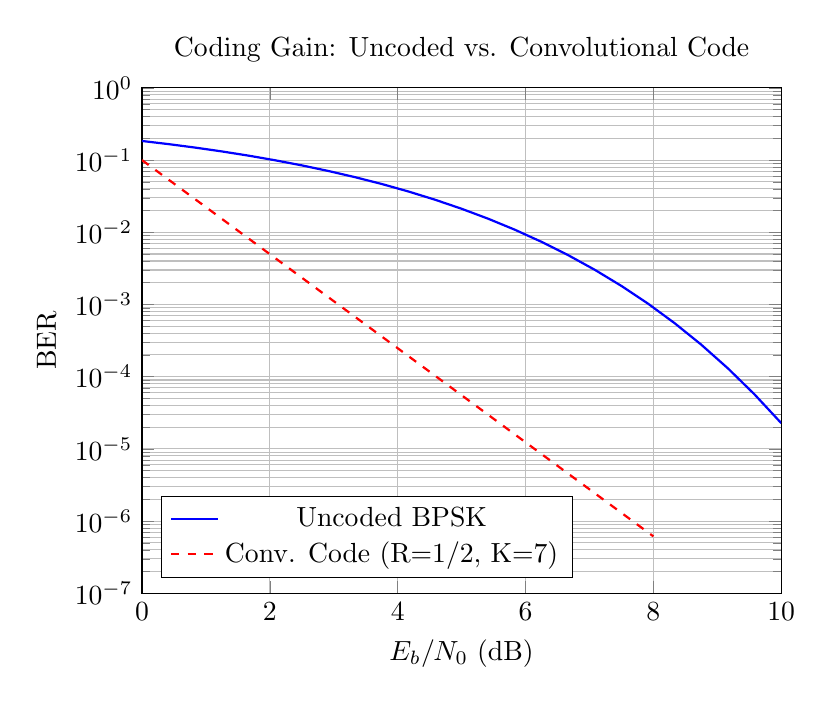
\begin{tikzpicture}
\begin{axis}[
    title={Coding Gain: Uncoded vs. Convolutional Code},
    xlabel={$E_b/N_0$ (dB)},
    ylabel={BER},
    ymode=log,
    grid=both,
    xmin=0, xmax=10,
    ymin=1e-7, ymax=1,
    width=0.8\textwidth,
    height=8cm,
    legend pos=south west
]
\addplot[blue, thick, domain=0:10] {0.5 * exp(-10^(x/10))};
\addlegendentry{Uncoded BPSK}
\addplot[red, thick, dashed, domain=0:8] {1e-1 * exp(-1.5*x)};
\addlegendentry{Conv. Code (R=1/2, K=7)}
\end{axis}
\end{tikzpicture}
\end{center}

\subsection{Soft-Decision Decoding}
Soft-decision decoding uses the analog values from the demodulator (rather than 0/1 bits) to calculate metrics. This provides a gain of approximately 2-3 dB over hard-decision decoding in AWGN channels.
